\clearpage

\section{EDFA}

\begin{tcolorbox}	
	\begin{tabular}{p{2.75cm} p{0.2cm} p{10.5cm}} 	
		\textbf{Header File}   &:& m\_qam\_receiver.h \\
		\textbf{Source File}   &:& m\_qam\_receiver.cpp \\
	\end{tabular}
\end{tcolorbox}

This block mimics  an EDFA in the simplest way, by accepting one optical input
signal and outputting an amplified version of that signal, affected by white
noise.

\begin{figure}[h]
	\centering
	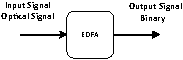
\includegraphics[width=0.5\textwidth]{./lib/edfa/figures/edfa_simple}
	\caption{Basic configuration of the MQAM
	receiver}\label{fig:edfa_simple}
\end{figure}

\subsection*{Functional description}

This block of code simulates the basic functionality of an EDFA: it amplifies
the optical signal by a given gain, and adds noise according to a certain noise
figure. Currently the only parameters are the gain and noise figure, and it's
assumed that the output power is always far below the EDFA's saturation
power. Therefore, the gain and noise spectral density are independent of the
signal. The noise spectral density is calculated from the noise
figure, gain and wavelength.

This block is made of smaller blocks, and its internal constitution is shown in
Figure~\ref{fig:edfa_blocks}.

\begin{figure}[h]
	\centering
	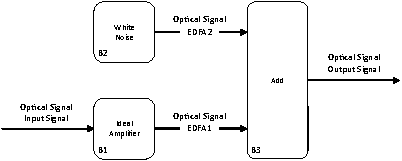
\includegraphics[width=0.7\textwidth]{./lib/edfa/figures/edfa_blocks}
	\caption{Schematic representation of the block homodyne
	receiver.}\label{fig:edfa_blocks}
\end{figure}

\subsection*{Input parameters}

%This block has some input parameters that can be manipulated by the user in
%order oto change the basic configuration of the receiver. Each parameter has
%associated a function that allows for its change. In the following table
%(table~\ref{table}) the input parameters and corresponding functions are
%summarized.
%
\begin{table}[h]
	\begin{center}
		\begin{tabular}{| m{3,2cm} | m{6,2cm} |  m{2,2cm} | m{4cm} | }
			\hline
			\textbf{Input parameters} & \textbf{Function} & \textbf{Type} \\\hline
			powerGain\_dB             & setGain\_dB       & t\_real       \\\hline
			noiseFigure               & setNoiseFigure    & t\_real       \\\hline
			samplingPeriod            & setNoiseFigure    & t\_real       \\\hline
			wavelength                & setWavelength     & t\_real       \\\hline
			dirName                   & setDirName        & string        \\\hline
		\end{tabular}
		\caption{List of input parameters of the EDFA block} \label{table}
	\end{center}
\end{table}
%
\pagebreak

\subsection*{Methods}

Edfa(vector<Signal *> \&inputSignal, vector<Signal *> \&outputSignal);
(\textbf{constructor})0
\bigbreak
void setGain\_dB(t\_real newGain)
\bigbreak
t\_real getGain\_dB(void)
\bigbreak
void setNoiseFigure(t\_real newNoiseFigure)
\bigbreak
t\_real getNoiseFigure(void)
\bigbreak
void setNoiseSamplingPeriod(t\_real newSamplingPeriod)
\bigbreak
t\_real getNoiseSamplingPeriod(void)
\bigbreak
void setWavelength(t\_real newWavelength)
\bigbreak
t\_real getNoiseFigure(void)
\bigbreak
void setDirName(string newDirName);
\bigbreak
string getDirName(void)
\bigbreak
%HomodyneReceiver(vector$<$Signal *$>$ \&inputSignal, vector$<$Signal *$>$
%\&outputSignal)
%\bigbreak
%void setIqAmplitudes(vector$<$t\_iqValues$>$ iqAmplitudesValues)
%\bigbreak
%vector$<$t\_iqValues$>$ const getIqAmplitudes(void)
%\bigbreak
%void setLocalOscillatorSamplingPeriod(double sPeriod)
%\bigbreak
%void setLocalOscillatorOpticalPower(double opticalPower)
%\bigbreak
%void setLocalOscillatorOpticalPower\_dBm(double opticalPower\_dBm)
%\bigbreak
%void setLocalOscillatorPhase(double lOscillatorPhase)
%\bigbreak
%void setLocalOscillatorOpticalWavelength(double lOscillatorWavelength)
%\bigbreak
%void setSamplingPeriod(double sPeriod)
%\bigbreak
%void  setResponsivity(t\_real Responsivity)
%\bigbreak
%void setAmplification(t\_real Amplification)
%\bigbreak
%void setNoiseAmplitude(t\_real NoiseAmplitude)
%\bigbreak
%void setImpulseResponseTimeLength(int impResponseTimeLength)
%\bigbreak
%void setFilterType(PulseShaperFilter fType)
%\bigbreak
%void setRollOffFactor(double rOffFactor)
%\bigbreak
%void setClockPeriod(double per)
%\bigbreak
%void setSamplesToSkip(int sToSkip)
%
%\pagebreak

\subsection*{Input Signals}

\subparagraph*{Number:} 1

\subparagraph*{Type:} Optical signal

\subsection*{Output Signals}

\subparagraph*{Number:} 1

\subparagraph*{Type:} Optical signal

\subsection*{Example}

\subsection*{Sugestions for future improvement}
